\documentclass{article}
\usepackage{verbatim}
\usepackage{vmargin}
\usepackage{graphicx,color}
\newcommand{\Note}[1]{{\bf \color{red}#1}}
\graphicspath{{./Figures/}}
\setpapersize{A4}
\usepackage{vmargin}
\setmargins
{2.5cm}                  % margen izquierdo
{1.5cm}                  % margen superior
{16.5cm}                 % anchura del texto
{23.42cm}                % altura del texto
{10pt}                   % altura de los encabezados
{1cm}                    % espacio entre el texto y los encabezados
{0pt}                    % altura del pie de página
{2cm}                    % espacio entre el texto y el pie de página

%%%%%%%%%%%%%%%%%%%%%%%%%%%%%%%%%%%%%%%%%%%%%%%%%%%%%%%%%%%%%%%%%%%%%%%%%%%%%%%%%%%%%%%%%%
%%%%%%%%%%%%%%%%%%%%%%%%%%%%%%%%%%%%%%%%%%%%%%%%%%%%%%%%%%%%%%%%%%%%%%%%%%%%%%%%%%%%%%%%%%
\title{Notes about the Coursera course \\ \textbf{Hadoop Platform and Application Framework}}
\author{Claudia Guti\'errez Escribano \\ Diego Duque Zumajo}
\begin{document}
\maketitle
\section*{\color{blue}Hadoop Basics\color{black}}
\subsection{Introduction}
The Apache Hadoop software library is a \textbf{framework that allows for the distributed processing of large data sets across clusters of computers using simple programming models}. It is designed to scale up from single servers to thousands of machines, each offering local computation and storage. Rather than rely on hardware to deliver high-availability, the library itself is designed to detect and handle failures at the application layer, so delivering a highly-available service on top of a cluster of computers, each of which may be prone to failures.\\
The key idea is to move computation to data, not data to computation. \\
The project includes these modules:
\begin{itemize}
\item Hadoop Common: The common utilities that \textbf{support the other Hadoop modules}. It contains the necessary Java ARchive (JAR) files and scripts needed to start Hadoop. 
\item Hadoop Distributed File System (HDFS): A distributed file system that provides high-throughput \textbf{access to application data}. See the HDFS comic (http://www.mail-archive.com/common-user@hadoop.apache.org/msg15171.html) for more information about how it works. 
\item Hadoop YARN: A framework for job scheduling and cluster resource \textbf{management}.
\item Hadoop MapReduce: A YARN-based system for \textbf{parallel processing of large data sets}.
\end{itemize}
%\begin{figure}[H]
%\centering
%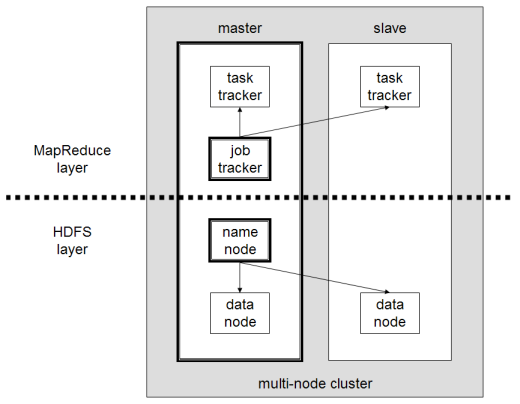
\includegraphics[scale=0.5]{Hadoop_1.png}
%\end{figure}
Other Hadoop-related projects at Apache, about them we will talk later, are: Hive, Pig, Spark, Zookeeper, HBase, etc.  
\subsection{Apache Sqoop}
Tool designed for efficiently transferring bulk data between Apache Hadoop and structure datastores such as relational databases. 
\subsection{Hbase}
Hbase is akey component of the Hadoop stack, as its design caters to applications that requieres really fast random access to significant data set.
\begin{itemize}
\item Column-oriented database management system. 
\item Key-value store. 
\item Based on Google big Table
\item Can hold extremely large data
\item Dynamic data model
\item Not a Relational DBMS.
\end{itemize}
\subsection{Pig}
It's a scripting language for creating MapReduce [1] programms using Hadoop. 
\begin{itemize}
\item Hihg level programming on top of Hadoop MaReduce. 
\item These language is called Pig Latin.
\item Data analysis problems as data flows. 
\end{itemize}
You can execute Pig scripts in other languages. 
\subsection{Hive}
Data warehouse software facilities queryng and managing large datasets residing in distribute storage. 
\subsection{Oozie}
Workflow scherudler system to manage Apache Hadoops jobs. Supports: MApReduce, Pig, Apache Hive, and Sqoop, etc. 
\subsection{Zookeeper}
\begin{itemize}
\item Provides operational services for a hadoop cluster. 
\item Centralized service for maintaining configuration information, naming, providing distributed synchronization, and providing. 
\end{itemize}
\subsection{Flume}
Distributed, reliable, and avaible service for efficiently collecting, aggregating, and moving large amount of data. 
\subsection{Spark}
A fast and general compute engine for Hadoop data. Spark provides a simple and expressive programming model that supports a wide range of applications, including ETL, machine learning, stream processing, and graph computation. Spark Benefits: 
\begin{itemize}
\item Multi-stage in-memory primitives provides performance up to 100 times faster for certain applications.
\item Allows user programs to load data into a cluster's memory and querit repeatedly. 
\item Well.suited to machine learning. 
\end{itemize}

\section*{\color{blue}Appendix\color{black}}
[1] \textbf{MapReduce} is a programming model and an associated implementation for processing and generating large data sets with a parallel, distributed algorithm on a cluster. \\
A MapReduce program is composed of a Map() procedure (method) that performs filtering and sorting (such as sorting students by first name into queues, one queue for each name) and a Reduce() method that performs a summary operation (such as counting the number of students in each queue, yielding name frequencies). \\
An example to understand how MapReduce works: 
\begin{verbatim}
function map(String name, String document):
  // name: document name
  // document: document contents
  for each word w in document:
    emit (w, 1)
\end{verbatim}
\begin{verbatim}
function reduce(String word, Iterator partialCounts):
  // word: a word
  // partialCounts: a list of aggregated partial counts
  sum = 0
  for each pc in partialCounts:
     sum += pc
  emit (word, sum)
\end{verbatim}
With this piece of code a document is split into words, and each word is counted by the \textit{ma}p function, using the word as a key. The framework put together all the pairs with the same key and feeds them to the same call to \textit{reduce}. so, this function only has to sum all its input to find the total appearances of that word. 

\end{document}
